\documentclass[11pt, a4paper]{article}

\usepackage[utf8]{inputenc} 
\usepackage[T1]{fontenc}    
\usepackage{lmodern}     
\usepackage{graphicx}  
\usepackage{booktabs}    
\usepackage{amsmath}      
\usepackage{cite}         
\usepackage{hyperref}      
% \usepackage[hyphens]{url}
\usepackage{multirow}
\usepackage{multicol}
\usepackage{subcaption}
\usepackage{cite}
\usepackage{amssymb}
\usepackage{tikz}
\usetikzlibrary{shapes.geometric, positioning, arrows.meta, calc}


\usepackage[a4paper, margin=1in]{geometry}


\usepackage{parskip} 



\title{Generative DeepSDF: Enhancing Implicit Shape Representation through Latent Vector Quantization}

\author{
    ARDACANDRA SUBIANTORO (G2505312G)
    \and   
    College of Computing and Data Science \\
    Nanyang Technological University, Singapore \\
    \texttt{ARDA0001@e.ntu.edu.sg}
}
\date{} 



\begin{document}

\maketitle

\begin{abstract}
Implicit neural representations, such as Signed Distance Functions (SDFs), excel at high-fidelity 3D shape reconstruction but struggle with probabilistic generation due to unconstrained continuous latent spaces. This research proposes Generative DeepSDF, which integrates a Vector Quantization (VQ) bottleneck into the DeepSDF architecture to discretize the latent manifold into a learned codebook of geometric features. A lightweight Autoregressive (AR) Transformer prior is then trained to model the distribution of these discrete sequences. Evaluations demonstrate that the VQ bottleneck preserves reconstruction fidelity while significantly improving latent space clustering. Furthermore, the AR prior enables the robust synthesis of novel 3D shapes, outperforming baseline continuous sampling in Minimum Matching Distance (MMD). The proposed framework successfully bridges deterministic implicit reconstruction and probabilistic generation, establishing a scalable foundation for 3D shape synthesis.
\end{abstract}


\section{Introduction}
Signed Distance Functions (SDFs) have emerged as a powerful continuous representation for 3D shapes. However, traditional frameworks like DeepSDF~\cite{Park_2019_CVPR} are primarily auto-decoder architectures designed for reconstruction. While they map shapes into a continuous latent space, this space is often poorly structured and unconstrained, making it difficult to generate new shapes. Simple interpolation or random sampling often results in physically impossible geometries. A solution is needed to bridge the gap between deterministic reconstruction and probabilistic generation within the implicit neural representation paradigm.

This research proposes the integration of Vector Quantization (VQ) into the DeepSDF pipeline. By replacing the standard continuous latent vector with a discrete, codebook-based bottleneck, each shape is represented as a collection of indices corresponding to learned prototypical geometric embeddings. This discretization effectively regularizes the latent manifold into a dictionary of reusable geometric features. By modeling the distribution of these discrete codes, it will result in more reliable generation of novel 3D shapes while maintaining the expressive power of implicit neural representations.

\section{Related Work}

\subsection{Neural Implicit Representations}
Traditional discrete representations of 3D geometry, such as point clouds, voxels, and meshes, often struggle with memory efficiency or topological constraints. DeepSDF~\cite{Park_2019_CVPR} represents a seminal shift toward continuous implicit functions parameterized by Multi-Layer Perceptrons (MLPs). In this framework, an MLP takes a spatial coordinate $\mathbf{x} \in \mathbb{R}^3$ and a shape-conditioned latent code $\mathbf{z}$ as input to predict a signed distance value. The 3D surface $\mathcal{M}$ is then implicitly defined as the zero-level set of the function:

\begin{equation}
\mathcal{M} = {\mathbf{x} \in \mathbb{R}^3 \mid f(\mathbf{x}, \mathbf{z}; \theta) = 0}
\end{equation}

While this approach enables high-fidelity reconstruction, the use of an auto-decoder with unconstrained latent vectors results in a manifold that lacks explicit structure. This makes it difficult to define robust category-level priors or perform high-quality probabilistic generation.

\subsection{Vector Quantization}
Vector Quantization (VQ) was popularized in the context of deep learning by the Neural Discrete Representation Learning (VQ-VAE) framework~\cite{oord2018neuraldiscreterepresentationlearning}. The key idea is instead of mapping input into a continuous Gaussian distribution, it introduces a discrete bottleneck by utilizing a learned codebook $\mathcal{C} = \{\mathbf{e}_1, \mathbf{e}_2, \dots, \mathbf{e}_K\}$, where each $\mathbf{e}_i \in \mathbb{R}^D$ represents a prototypical embedding vector in a $D$-dimensional space.

In this architecture, an encoder produces a continuous latent representation $\mathbf{z}_e(x)$. This vector is then quantized by mapping it to the nearest entry in the codebook based on Euclidean distance:\begin{equation}\mathbf{z}_q(x) = \mathbf{e}_k, \quad \text{where } k = \arg\min_j |\mathbf{z}_e(x) - \mathbf{e}_j|_2\end{equation}

Discretizing the latent space offers several key advantages. It forces the model to ignore high-frequency noise in favor of a robust dictionary of geometric features. Additionally, it prevents posterior collapse, ensuring that the latent space remains informative and well-structured throughout training.

\subsection{Generative 3D Shape Synthesis}
The most related work to this report is AutoSDF~\cite{mittal2023autosdfshapepriors3d}, which addresses the generative limitations of DeepSDF by discretizing volumetric T-SDFs into a symbolic latent grid via a 3D-VQ-VAE. The framework introduces Patch-wise Encoding (P-VQ-VAE) to independently encode local regions, ensuring that latent codes for partial observations remain consistent with full-shape representations. This localized encoding is paired with joint decoding to preserve global structural coherence. By modeling this discrete space with a non-sequential Transformer prior, AutoSDF enables expressive, multi-modal shape synthesis and flexible conditioning on arbitrary spatial query locations. Generative DeepSDF serves as a lightweight version of AutoSDF by simplifying its complex 3D patch-based grid into a 1D sequence of 16 quantized latent groups, allowing it to synthesize novel 3D shapes from implicit functions using a compact sequential prior.


\section{Method}

\subsection{Dataset Selection}
This experiment utilizes a subset of the ShapeNet~\cite{shapenet2015} dataset. Three specific object categories are selected: "Chair", "Table", and "Airplane". The "Chair" and "Table" categories are chosen because these objects share common structural features, such as legs and planar surfaces, yet possess distinct global topologies. This selection is intended to challenge the vector quantization process to differentiate between visually similar local features while effectively separating categorically distinct geometries within the latent manifold. In contrast, the "Airplane" category offers a fundamentally different geometric profile, which is expected to occupy a region of the latent space far removed from the other categories. 50 objects per category are randomly selected for this experiment.

\subsection{Data Preprocessing}
The ShapeNet dataset provides the meshes of the 3D objects, but not the SDF values. Some preprocessing steps are required to calculate the ground-truth SDF. Each mesh is first scaled to fit within a unit sphere to ensure comparable coordinates. For each scaled mesh, 500,000 spatial points are sampled, with higher density near the object surface. Near-surface points are generated by offsetting along outward-facing surface normals, with the normal orientation determined by trimesh's precomputed face normals and a global radial alignment check. SDF values are then computed: for watertight meshes, inside/outside sign is determined directly via a ray-casting containment test; for non-watertight meshes, a k-nearest neighbor voting scheme is used, where the sign is estimated from distance-weighted projections onto the normals of the 21 nearest surface samples.

\begin{figure}[htbp]
    \centering
    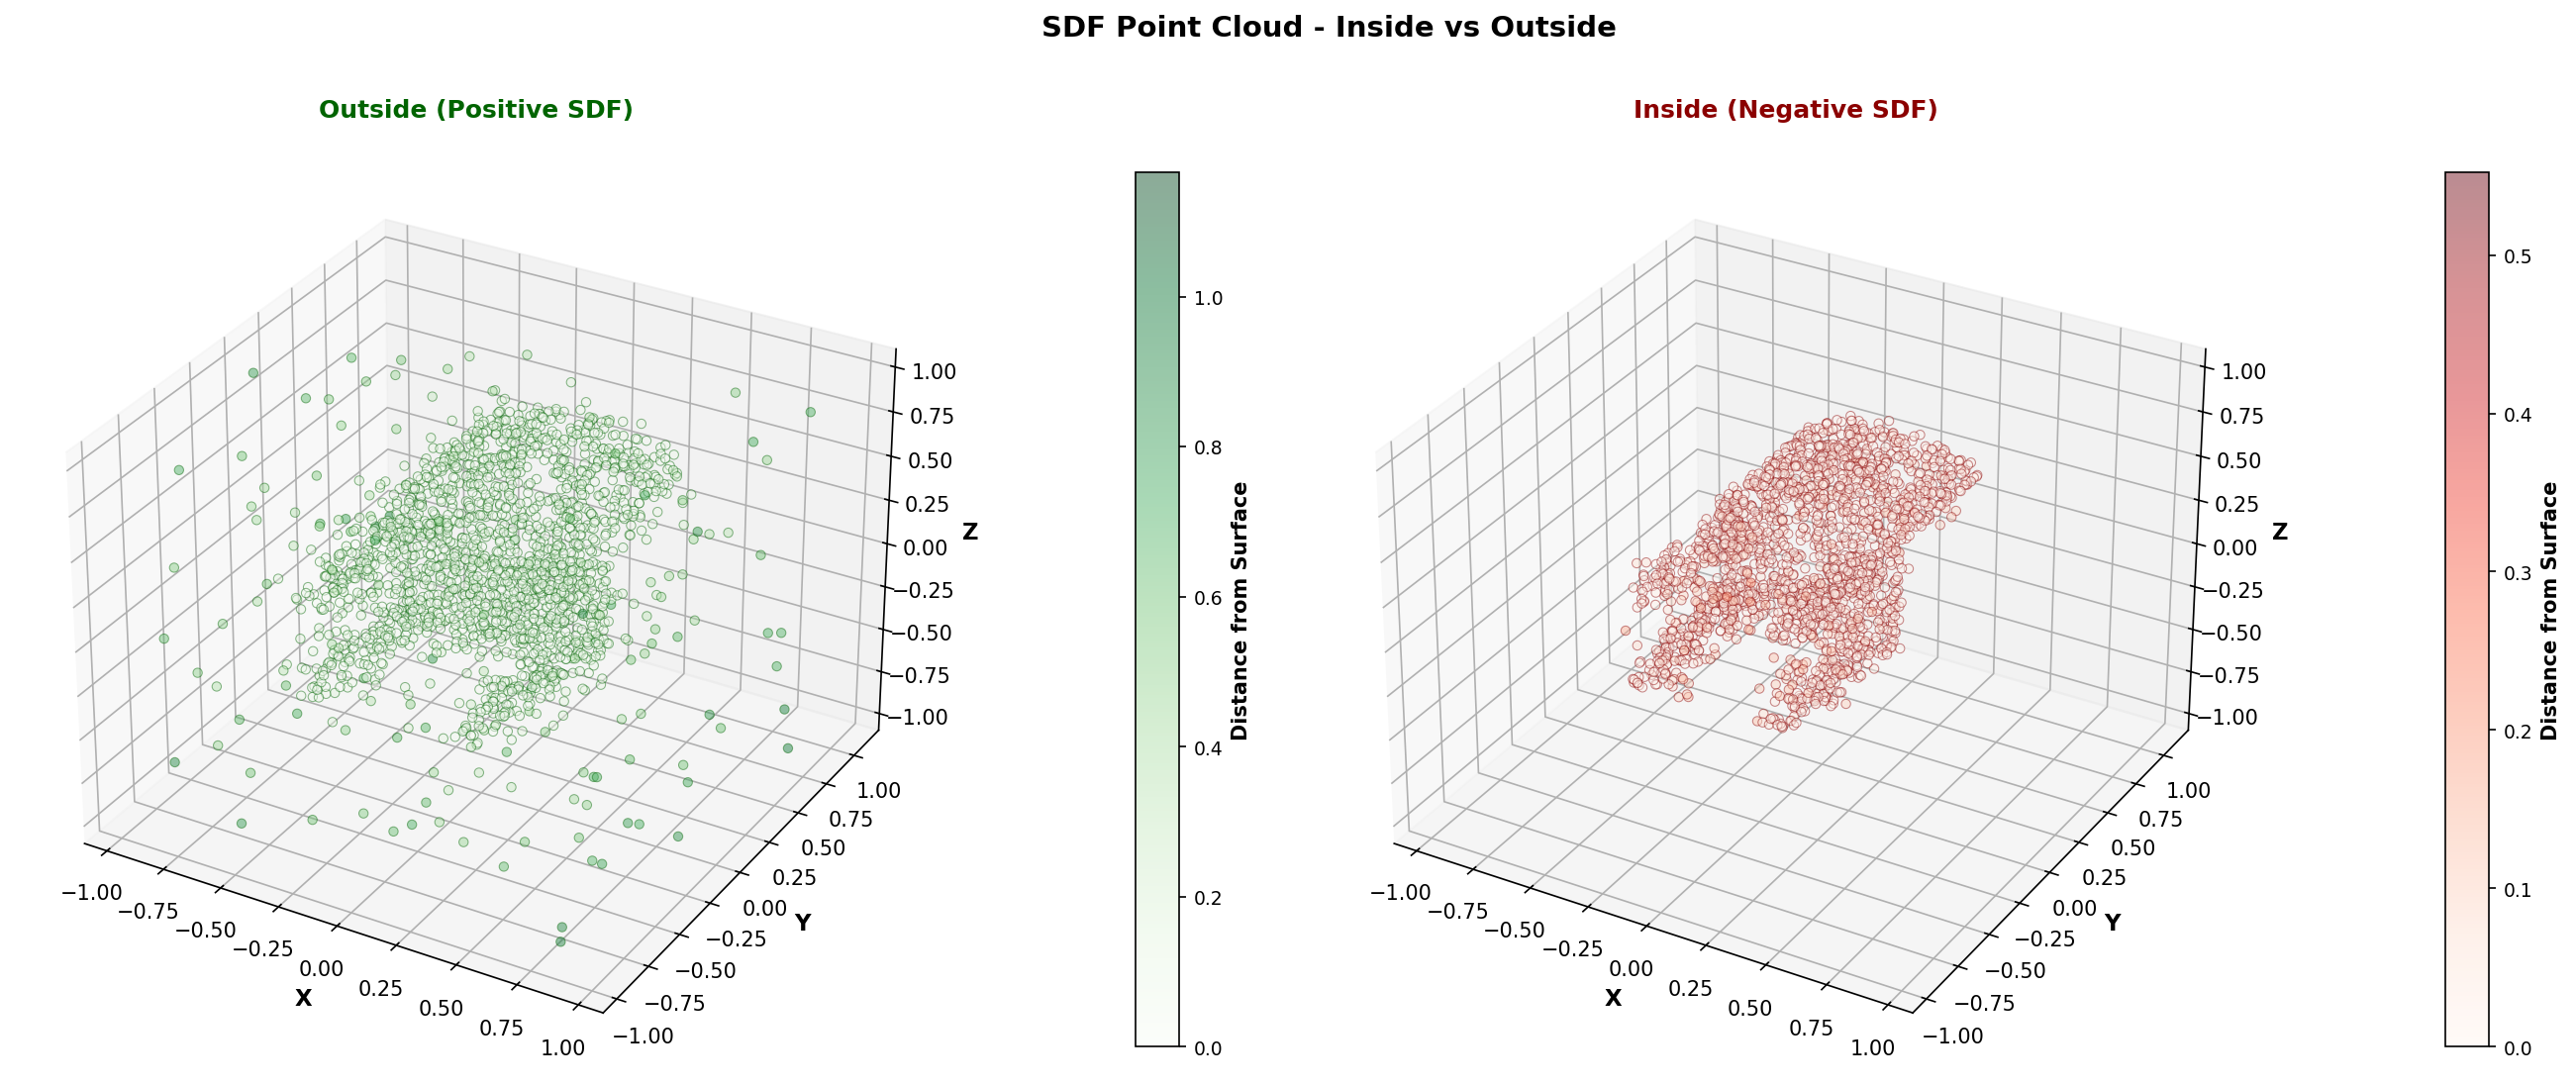
\includegraphics[width=0.8\linewidth]{img/chair_3d_scatter.png}
    \caption{Sample SDF preprocessing output for category "Chair".}
    \label{fig:preprocessing_output}
\end{figure}

\subsection{Baseline Architecture}

% \begin{figure}[htbp]
%     \centering
%     \includegraphics[width=0.8\linewidth]{img/deepsdf_baseline_architecture.png}
%     \caption{Model architecture diagram for the baseline DeepSDF.}
%     \label{fig:deepsdf_architecture}
% \end{figure}

\begin{figure}[htbp]
    \centering
    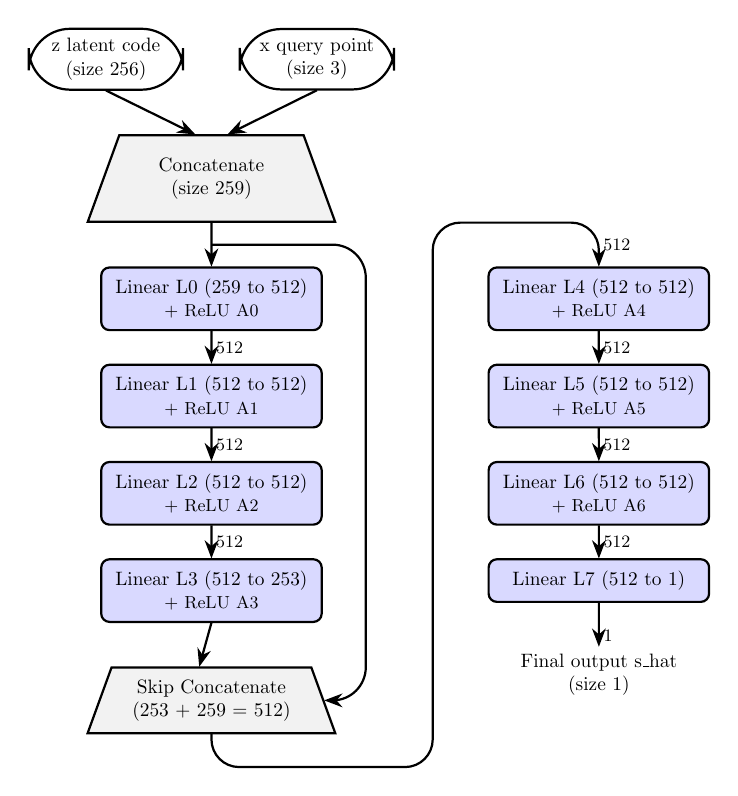
\begin{tikzpicture}[
        scale=0.70, transform shape,
        % Define styles for the nodes
        base_node/.style={draw, align=center, rounded corners=3pt, thick},
        layer/.style={base_node, fill=blue!15, minimum width=4cm, inner sep=6pt},
        input_node/.style={base_node, fill=white, minimum width=2.8cm, inner sep=5pt, rounded corners=15pt},
        concat_node/.style={trapezium, trapezium left angle=70, trapezium right angle=70, draw, fill=gray!10, minimum width=4.5cm, inner sep=4pt, align=center, thick},
        arrow/.style={-Stealth, thick},
        dim_label/.style={pos=0.5, right, inner sep=2pt, font=\small}
    ]

    % ==============================================
    % === SCOPE FOR LEFT COLUMN (Inputs, L0-L3) ===
    % ==============================================
    \begin{scope}
        
        % Place input nodes
        \node (z_input) [input_node] {z latent code\\(size 256)};
        \node (x_input) [input_node, right=1cm of z_input] {x query point\\(size 3)};

        % Place first concatenation block
        \node (concat1) [concat_node, below=0.8cm of $(z_input.south)!0.5!(x_input.south)$] {Concatenate\\(size 259)};

        % Connect inputs to concat1
        \draw [arrow] (z_input.south) -- (concat1.110);
        \draw [arrow] (x_input.south) -- (concat1.70);

        % Start of Left Column (L0-L3)
        \node (L0) [layer, below=0.8cm of concat1] {Linear L0 (259 to 512) \\ \small + ReLU A0};
        \draw [arrow] (concat1.south) -- (L0);

        \node (L1) [layer, below=0.6cm of L0] {Linear L1 (512 to 512) \\ \small + ReLU A1};
        \draw [arrow] (L0.south) -- node [dim_label] {512} (L1);

        \node (L2) [layer, below=0.6cm of L1] {Linear L2 (512 to 512) \\ \small + ReLU A2};
        \draw [arrow] (L1.south) -- node [dim_label] {512} (L2);

        \node (L3) [layer, below=0.6cm of L2] {Linear L3 (512 to 253) \\ \small + ReLU A3};
        \draw [arrow] (L2.south) -- node [dim_label] {512} (L3);

        % Place second concatenation block
        \node (concat2) [concat_node, below=0.8cm of L3] {Skip Concatenate\\(253 + 259 = 512)};
        \draw [arrow] (L3.south) -- (concat2.110);

        % Draw skip connection tightly in the middle gap
        \path (concat1.south) -- coordinate[pos=0.5] (branch_pt) (L0.north);
        \draw [arrow, rounded corners=12pt] (branch_pt) -- ++(2.8cm,0) |- node[pos=0.25, right, inner sep=4pt] {} (concat2.east);
        
    \end{scope}

    % ===============================================
    % === SCOPE FOR RIGHT COLUMN (L4-L8, Output) ===
    % ===============================================
    \begin{scope}
        
        % Bridge to the right column
        % Changed positioning from "below of concat2" to "right of L0"
        \node (L4) [layer, right=3cm of L0] {Linear L4 (512 to 512) \\ \small + ReLU A4};
        
        % Bridging arrow traveling up the gap between the columns
        \draw [arrow, rounded corners=10pt] (concat2.south) -- ++(0,-0.6cm) -| ([xshift=-1cm]L4.west) |- ([yshift=0.8cm]L4.north) -- node [dim_label] {512} (L4.north);

        % Continue with the right column (L5-L8)
        \node (L5) [layer, below=0.6cm of L4] {Linear L5 (512 to 512) \\ \small + ReLU A5};
        \draw [arrow] (L4.south) -- node [dim_label] {512} (L5);

        \node (L6) [layer, below=0.6cm of L5] {Linear L6 (512 to 512) \\ \small + ReLU A6};
        \draw [arrow] (L5.south) -- node [dim_label] {512} (L6);

        \node (L7) [layer, below=0.6cm of L6] {Linear L7 (512 to 1)};
        \draw [arrow] (L6.south) -- node [dim_label] {512} (L7);

        % \node (L8) [layer, below=0.6cm of L7] {Linear L8 (512 to 1)};
        % \draw [arrow] (L7.south) -- node [dim_label] {512} (L8);

        % Final output
        \node (final) [below=0.8cm of L7, align=center] {Final output s\_hat\\(size 1)};
        \draw [arrow] (L7.south) -- node [dim_label, near end] {1} (final.north);
        
    \end{scope}

    \end{tikzpicture}
    
    \caption{Model architecture diagram for the baseline DeepSDF.}
    \label{fig:deepsdf_architecture}
\end{figure}

A standard DeepSDF auto-decoder is used as the baseline for this experiment. Each distinct shape $i$ is assigned a latent code $\mathbf{z}_i \in \mathbb{R}^d$. The latent code $\mathbf{z}_i$ and the 3D coordinate $\mathbf{x} \in \mathbb{R}^3$ are concatenated and taken as the input to the DeepSDF auto-decoder MLP. The decoder is an MLP with 8 hidden layers of width 512, ReLU activations, and a skip connection that re-injects the original input at an intermediate layer. The loss function is a clamped $L_1$ loss between the predicted signed distance and the ground-truth value $s$. Furthermore, a latent-norm penalty is applied to ensure that the distribution of latent codes remains compact and well-regularized on the manifold: 

\begin{equation}
    \mathcal{L}{sdf} = |clamp(f\theta(\mathbf{z}_i, \mathbf{x}), \delta) - clamp(s, \delta)| + \lambda_z |\mathbf{z}_i|_2
\end{equation}

where $s$ is the ground-truth signed distance value and $\delta$ is the clamping threshold.

\subsection{Latent Vector Quantization}

The proposed model extends the DeepSDF auto-decoder by introducing a vector quantization (VQ) bottleneck between the per-shape latent codes and the decoder. The decoder architecture is identical to the baseline: an 8-layer MLP of width 512 with weight-normalized linear layers, ReLU activations, a skip connection at layer 4, and a final Tanh activation.

\begin{figure}[htbp]
    \centering
    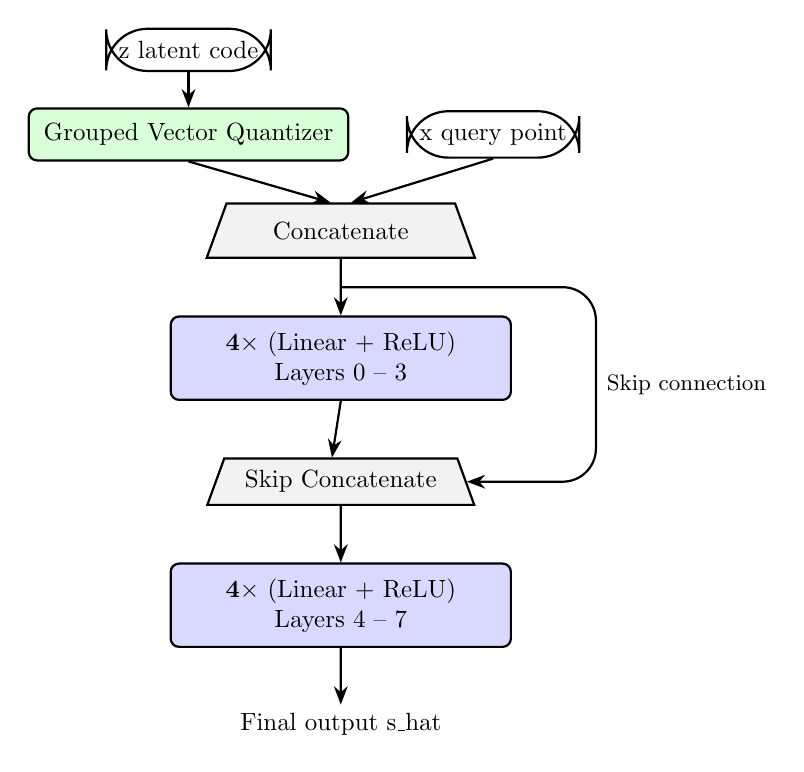
\begin{tikzpicture}[
        % Scale down slightly for a perfect fit
        scale=0.9, transform shape,
        % Define styles for the nodes
        base_node/.style={draw, align=center, rounded corners=3pt, thick},
        layer/.style={base_node, fill=blue!15, minimum width=4.8cm, inner sep=6pt},
        input_node/.style={base_node, fill=white, minimum width=2.2cm, inner sep=5pt, rounded corners=15pt},
        concat_node/.style={trapezium, trapezium left angle=70, trapezium right angle=70, draw, fill=gray!10, minimum width=3.8cm, inner sep=4pt, align=center, thick},
        vq_node/.style={base_node, fill=green!15, minimum width=3.2cm, inner sep=6pt},
        arrow/.style={-Stealth, thick}
    ]

    % Place z input
    \node (z_input) [input_node] {z latent code};
    
    % Grouped Vector Quantizer Block
    \node (vq) [vq_node, below=0.5cm of z_input] {Grouped Vector Quantizer};
    \draw [arrow] (z_input.south) -- (vq.north);

    % Place x input aligned horizontally with the VQ block
    \node (x_input) [input_node, right=0.8cm of vq] {x query point};

    % Place first concatenation block
    \node (concat1) [concat_node, below=0.6cm of $(vq.south)!0.5!(x_input.south)$] {Concatenate};

    % Connect quantized z and x to concat1
    \draw [arrow] (vq.south) -- (concat1.110);
    \draw [arrow] (x_input.south) -- (concat1.70);

    % MACRO BLOCK 1: Layers 0 to 3
    \node (L0_3) [layer, below=0.8cm of concat1] {\textbf{4$\times$} (Linear + ReLU) \\ Layers 0 -- 3};
    \draw [arrow] (concat1.south) -- (L0_3);

    % Place second concatenation block
    \node (concat2) [concat_node, below=0.8cm of L0_3] {Skip Concatenate};
    \draw [arrow] (L0_3.south) -- (concat2.110);

    % Draw skip connection tightly looping around the first block
    \path (concat1.south) -- coordinate[pos=0.5] (branch_pt) (L0_3.north);
    \draw [arrow, rounded corners=12pt] (branch_pt) -- ++(3.6cm,0) |- node[pos=0.25, right, inner sep=4pt] {\small Skip connection} (concat2.east);
    
    % MACRO BLOCK 2: Layers 4 to 7
    \node (L4_7) [layer, below=0.8cm of concat2] {\textbf{4$\times$} (Linear + ReLU) \\ Layers 4 -- 7};
    \draw [arrow] (concat2.south) -- (L4_7);

    % Final output directly below the second block
    \node (final) [below=0.8cm of L4_7, align=center] {Final output s\_hat};
    \draw [arrow] (L4_7.south) -- (final.north);

    \end{tikzpicture}
    
    \caption{Generative DeepSDF architecture featuring Latent Vector Quantization.}
    \label{fig:vq_deepsdf_architecture}
\end{figure}

\subsubsection{Vector Quantization Bottleneck}
Each shape $i$ still maintains a continuous latent code $\mathbf{z}_i^e \in \mathbb{R}^{256}$, which is passed through a grouped vector quantizer before being fed to the decoder. The latent vector is split into $G = 16$ equal groups of dimension $d_c = 16$ (so that $G \times d_c = 256$), and each group is independently quantized to its nearest entry in a separate codebook $\mathbf{C}^g \in \mathbb{R}^{K \times d_c}$, where $K = 24$ is the codebook size. The quantized vector is reconstructed by concatenating the $G$ selected entries:

\begin{equation}
    \mathbf{z}_i^q = \bigoplus_{g=1}^{G}\, \mathbf{c}^g_{k^*},
    \quad k^* = \arg\min_{k}\, \|\mathbf{z}_i^{e,g} - \mathbf{c}^g_k\|_2^2
\end{equation}

where $\mathbf{z}_i^{e,g}$ denotes the $g$-th group of the continuous latent and $\bigoplus$ denotes concatenation. The decoder receives the quantized vector $\mathbf{z}_i^q$ instead of $\mathbf{z}_i^e$.

\subsubsection{Straight-Through Gradient Estimation}
Since the $\arg\min$ operation is non-differentiable, gradients are passed straight through the quantizer to the continuous latents using the straight-through estimator:

\begin{equation}
    \mathbf{z}_i^{st} = \mathbf{z}_i^e + \bigl(\mathbf{z}_i^q - \mathbf{z}_i^e\bigr)^{\mathrm{sg}}
\end{equation}

where $(\cdot)^{\mathrm{sg}}$ denotes the stop-gradient operator.

\begin{figure}[htbp]
    \centering
    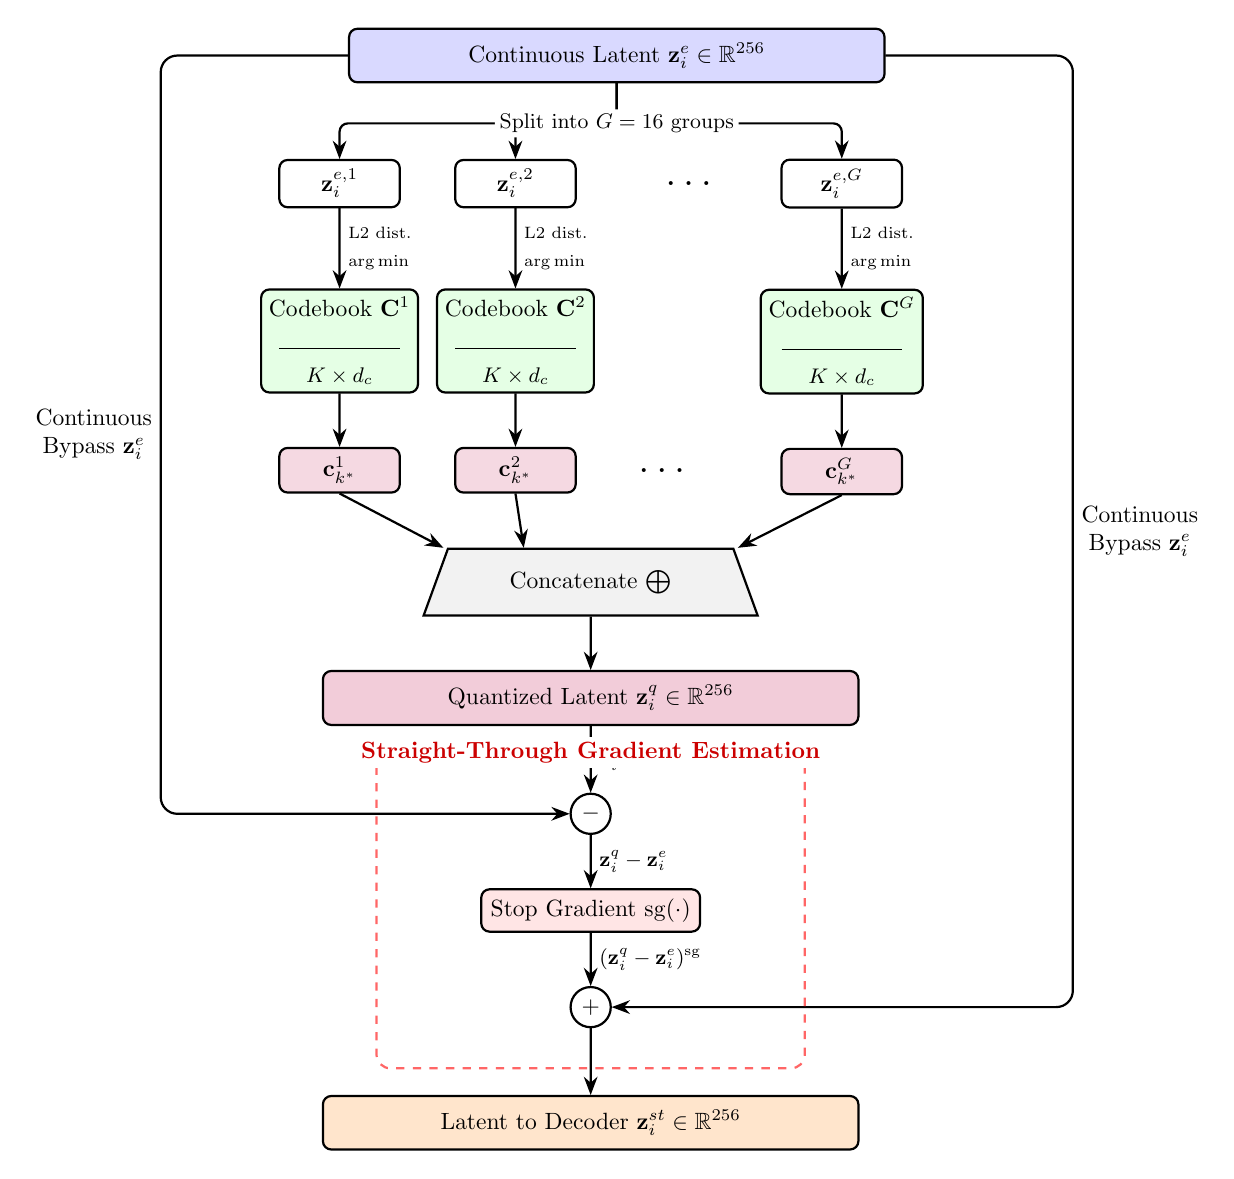
\begin{tikzpicture}[
        % Scaling and standard setup
        scale=0.85, transform shape,
        base_node/.style={draw, thick, align=center, rounded corners=3pt},
        latent_node/.style={base_node, fill=blue!15, minimum width=8cm, inner sep=6pt},
        group_node/.style={base_node, fill=white, minimum width=1.8cm, inner sep=4pt},
        codebook_node/.style={base_node, fill=green!10, minimum width=2cm, minimum height=1.5cm},
        quant_node/.style={base_node, fill=purple!15, minimum width=1.8cm, inner sep=4pt},
        concat_node/.style={trapezium, trapezium left angle=70, trapezium right angle=70, draw, fill=gray!10, minimum width=5cm, inner sep=4pt, thick},
        op_node/.style={draw, circle, thick, fill=white, inner sep=1pt, minimum width=0.6cm},
        sg_node/.style={base_node, fill=red!10, inner sep=4pt, minimum width=3cm},
        arrow/.style={-Stealth, thick}
    ]

    % ==========================================
    % 1. CONTINUOUS LATENT INPUT
    % ==========================================
    \node (ze) [latent_node] {Continuous Latent $\mathbf{z}_i^e \in \mathbb{R}^{256}$};

    % ==========================================
    % 2. SPLIT INTO GROUPS
    % ==========================================
    \coordinate (split_center) at ($(ze.south) + (0, -1.5cm)$);
    
    \node (g2) [group_node, left=0.6cm of split_center] {$\mathbf{z}_i^{e,2}$};
    \node (g1) [group_node, left=0.8cm of g2] {$\mathbf{z}_i^{e,1}$};
    \node (dots1) [right=0.6cm of split_center] {\LARGE $\dots$};
    \node (gG) [group_node, right=0.8cm of dots1] {$\mathbf{z}_i^{e,G}$};

    % Branching arrows for the split (using rounded corners to form a single trunk)
    \draw [arrow, rounded corners=3pt] (ze.south) -- ++(0, -0.6cm) -| (g1.north);
    \draw [arrow, rounded corners=3pt] (ze.south) -- ++(0, -0.6cm) -| (g2.north);
    \draw [arrow, rounded corners=3pt] (ze.south) -- ++(0, -0.6cm) -| (gG.north);
    \node [fill=white, inner sep=2pt, rounded corners=2pt] at ($(ze.south) + (0, -0.6cm)$) {\small Split into $G=16$ groups};

    % ==========================================
    % 3. VECTOR QUANTIZATION (CODEBOOKS)
    % ==========================================
    % FIXED: Replaced \hrule with \rule{width}{height} inside the nodes
    \node (cb1) [codebook_node, below=1.2cm of g1] {Codebook $\mathbf{C}^1$\\[2pt] \rule{1.8cm}{0.4pt} \\[2pt] \small $K \times d_c$};
    \node (cb2) [codebook_node, below=1.2cm of g2] {Codebook $\mathbf{C}^2$\\[2pt] \rule{1.8cm}{0.4pt} \\[2pt] \small $K \times d_c$};
    \node (cbG) [codebook_node, below=1.2cm of gG] {Codebook $\mathbf{C}^G$\\[2pt] \rule{1.8cm}{0.4pt} \\[2pt] \small $K \times d_c$};

    % Arrows with argmin equations
    \draw [arrow] (g1.south) -- node[right, align=left] {\scriptsize L2 dist.\\\scriptsize $\arg\min$} (cb1.north);
    \draw [arrow] (g2.south) -- node[right, align=left] {\scriptsize L2 dist.\\\scriptsize $\arg\min$} (cb2.north);
    \draw [arrow] (gG.south) -- node[right, align=left] {\scriptsize L2 dist.\\\scriptsize $\arg\min$} (cbG.north);

    % ==========================================
    % 4. EXTRACTED QUANTIZED VECTORS
    % ==========================================
    \node (q1) [quant_node, below=0.8cm of cb1] {$\mathbf{c}^1_{k^*}$};
    \node (q2) [quant_node, below=0.8cm of cb2] {$\mathbf{c}^2_{k^*}$};
    \node (dots2) [right=0.8cm of q2] {\LARGE $\dots$};
    \node (qG) [quant_node, below=0.8cm of cbG] {$\mathbf{c}^G_{k^*}$};

    \draw [arrow] (cb1.south) -- (q1.north);
    \draw [arrow] (cb2.south) -- (q2.north);
    \draw [arrow] (cbG.south) -- (qG.north);

    % ==========================================
    % 5. CONCATENATION BOTTLENECK
    % ==========================================
    \coordinate (concat_center) at ($(q1.south)!0.5!(qG.south)$);
    \node (concat) [concat_node, below=0.8cm of concat_center] {Concatenate $\bigoplus$};
    
    % Converging arrows for concatenation
    \draw [arrow] (q1.south) -- ([xshift=-2.2cm]concat.north);
    \draw [arrow] (q2.south) -- ([xshift=-1cm]concat.north);
    \draw [arrow] (qG.south) -- ([xshift=2.2cm]concat.north);

    % Quantized Output
    \node (zq) [latent_node, fill=purple!20, below=0.8cm of concat] {Quantized Latent $\mathbf{z}_i^q \in \mathbb{R}^{256}$};
    \draw [arrow] (concat.south) -- (zq.north);

    % ==========================================
    % 6. STRAIGHT-THROUGH ESTIMATOR (STE)
    % ==========================================
    
    % Subtraction Node
    \node (minus) [op_node, below=1cm of zq] {$-$};
    \draw [arrow] (zq.south) -- node[right] {\small $\mathbf{z}_i^q$} (minus.north);

    % Stop Gradient Node
    \node (sg) [sg_node, below=0.8cm of minus] {Stop Gradient $\mathrm{sg}(\cdot)$};
    \draw [arrow] (minus.south) -- node[right] {\small $\mathbf{z}_i^q - \mathbf{z}_i^e$} (sg.north);

    % Addition Node
    \node (plus) [op_node, below=0.8cm of sg] {$+$};
    \draw [arrow] (sg.south) -- node[right] {\small $(\mathbf{z}_i^q - \mathbf{z}_i^e)^{\mathrm{sg}}$} (plus.north);

    % Final STE Output
    \node (zst) [latent_node, fill=orange!20, below=1cm of plus] {Latent to Decoder $\mathbf{z}_i^{st} \in \mathbb{R}^{256}$};
    \draw [arrow] (plus.south) -- (zst.north);

    % --- The Bypass Skip Connections for z^e ---
    % Routes z^e down the left side to the subtraction node
    \draw [arrow, rounded corners=6pt] (ze.west) -- ++(-2.8cm, 0) |- 
        node[pos=0.25, left, align=center] {Continuous\\Bypass $\mathbf{z}_i^e$} (minus.west);
        
    % Routes z^e down the right side to the addition node
    \draw [arrow, rounded corners=6pt] (ze.east) -- ++(2.8cm, 0) |- 
        node[pos=0.25, right, align=center] {Continuous\\Bypass $\mathbf{z}_i^e$} (plus.east);

    % --- Visual bounding box for the STE block ---
    \draw [thick, dashed, red!60, rounded corners=5pt] 
        ($(minus.north) + (-3.2cm, 0.6cm)$) rectangle ($(plus.south) + (3.2cm, -0.6cm)$);
    \node [text=red!80!black, font=\bfseries, fill=white, inner sep=2pt] 
        at ($(minus.north) + (0, 0.6cm)$) {Straight-Through Gradient Estimation};

    \end{tikzpicture}
    
    \caption{Visualization of the Grouped Vector Quantizer and Straight-Through Estimator. The continuous latent $\mathbf{z}_i^e$ is split into $G=16$ groups, quantized against independent codebooks, and concatenated into $\mathbf{z}_i^q$. Gradients bypass the non-differentiable $\arg\min$ operation via the STE computational graph.}
    \label{fig:vq_and_ste}
\end{figure}

\subsubsection{Training Objective}
The full training loss is:

\begin{equation}
    \mathcal{L} = \mathcal{L}_{\mathrm{sdf}} + \beta_{\mathrm{cm}}\,\mathcal{L}_{\mathrm{commit}} - \beta_{\mathrm{ent}}\,\mathcal{H}
\end{equation}

where:

\begin{align}
    \mathcal{L}_{\mathrm{sdf}} &= \bigl|\,\mathrm{clamp}(f_\theta(\mathbf{z}_i^{st},\, \mathbf{x}),\, \delta) - \mathrm{clamp}(s,\, \delta)\,\bigr| \\
    \mathcal{L}_{\mathrm{commit}} &= \bigl\|(\mathbf{z}_i^q)^{\mathrm{sg}} - \mathbf{z}_i^e\bigr\|_2^2 \\
    \mathcal{H} &= -\sum_k \bar{u}_k \log(\bar{u}_k)
\end{align}

Codebook entries are updated via Exponential Moving Averages of assigned encoder outputs rather than a gradient loss, improving stability on small datasets. Dead codes are periodically reseeded with random encoder outputs to prevent collapse. $\mathcal{L}_{\mathrm{commit}}$ encourages the encoder to commit to codebook entries, $\mathcal{H}$ is the entropy of average codebook usage maximized to encourage uniform code utilization, and $\beta_{\mathrm{cm}}$, $\beta_{\mathrm{ent}}$ are their respective weights. Unlike the baseline, no latent-norm regularization is applied, as the VQ bottleneck itself constrains the latent space.

\subsection{Generative Prior for Novel Shape Synthesis}
While the vector quantization bottleneck discretizes the latent space, it does not inherently learn the joint probability distribution of these geometric features. To enable the synthesis of novel shapes, a generative prior must be trained over the quantized latent space to model valid codebook combinations.

Given the limited dataset size, high-capacity models (e.g., deep Transformers or discrete diffusion) risk overfitting by memorizing specific training sequences. Therefore, a lightweight, 3-layer autoregressive (AR) Transformer is employed. The grouped vector quantizer already partitions the latent space into a fixed-length sequence of $G=16$ discrete tokens. The AR prior models the probability of this sequence $\mathbf{z}^q$ as:$$p(\mathbf{z}^q) = \prod_{g=1}^{G} p(\mathbf{c}^g \mid \mathbf{c}^1, \dots, \mathbf{c}^{g-1})$$

The architecture maps the $K=24$ codebook indices to learned embeddings, combined with positional encodings to preserve structural order. A high dropout rate is applied to the causal attention layers to force the model to learn generalizable categorical grammar rather than high-frequency noise.

During training, the auto-decoder and VQ codebooks are strictly frozen. The prior is trained using a standard multi-class cross-entropy loss to predict the next token in the sequence. At inference, novel shapes are generated by autoregressively sampling tokens step-by-step from the predicted distributions, which are then passed to the auto-decoder for continuous SDF reconstruction.

\begin{figure}[htbp]
    \centering
    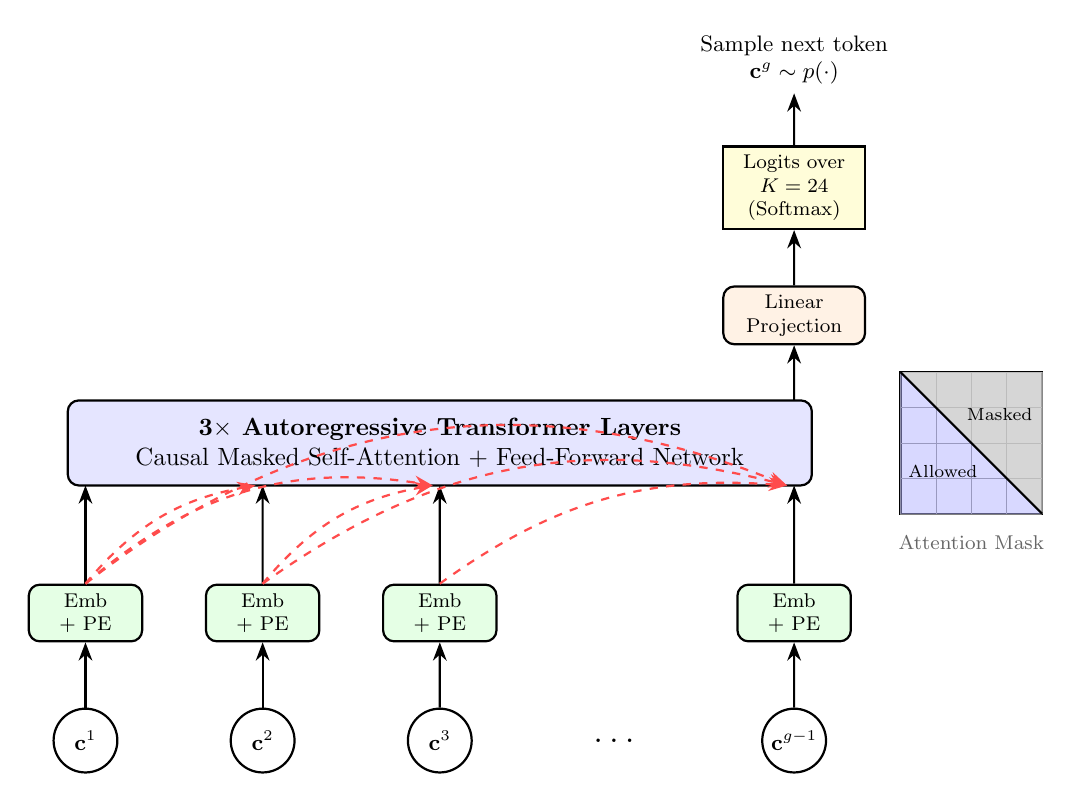
\begin{tikzpicture}[
        scale=0.9, transform shape,
        % Define styles
        token/.style={draw, circle, thick, fill=white, minimum size=0.9cm, inner sep=0pt, font=\small},
        layer/.style={draw, thick, rounded corners, fill=green!10, minimum width=1.6cm, minimum height=0.8cm, align=center, font=\footnotesize},
        attn/.style={draw, thick, rounded corners, fill=blue!10, minimum width=10.5cm, minimum height=1.2cm, align=center},
        outlayer/.style={draw, thick, rounded corners, fill=orange!10, minimum width=2cm, minimum height=0.8cm, align=center, font=\footnotesize},
        arrow/.style={->, >=Stealth, thick},
        causal/.style={->, >=Stealth, thick, dashed, red!70}
    ]

    % 1. Input Tokens
    \node[token] (c1) at (0, 0) {$\mathbf{c}^1$};
    \node[token] (c2) at (2.5, 0) {$\mathbf{c}^2$};
    \node[token] (c3) at (5, 0) {$\mathbf{c}^3$};
    \node at (7.5, 0) {\Large $\dots$};
    \node[token] (cg) at (10, 0) {$\mathbf{c}^{g-1}$};

    % 2. Embedding + Positional Encoding Layer
    \node[layer] (e1) at (0, 1.8) {Emb \\ + PE};
    \node[layer] (e2) at (2.5, 1.8) {Emb \\ + PE};
    \node[layer] (e3) at (5, 1.8) {Emb \\ + PE};
    \node[layer] (eg) at (10, 1.8) {Emb \\ + PE};

    % Arrows from tokens to embeddings
    \draw[arrow] (c1) -- (e1);
    \draw[arrow] (c2) -- (e2);
    \draw[arrow] (c3) -- (e3);
    \draw[arrow] (cg) -- (eg);

    % 3. Main Transformer Block
    \node[attn] (tf) at (5, 4.2) {\textbf{3$\times$ Autoregressive Transformer Layers} \\ Causal Masked Self-Attention + Feed-Forward Network};

    % Straight vertical paths into the Transformer block
    \draw[arrow] (e1.north) -- (0, 3.6);
    \draw[arrow] (e2.north) -- (2.5, 3.6);
    \draw[arrow] (e3.north) -- (5, 3.6);
    \draw[arrow] (eg.north) -- (10, 3.6);

    % Causal Dependency Arrows (Curved, Dashed, Red)
    % c^1 attends to itself (straight line) and influences future tokens:
    \draw[causal] (e1.north) to[bend left=20] (2.4, 3.6);
    \draw[causal] (e1.north) to[bend left=25] (4.9, 3.6);
    \draw[causal] (e1.north) to[bend left=30] (9.9, 3.6);

    % c^2 influences future tokens:
    \draw[causal] (e2.north) to[bend left=20] (4.9, 3.6);
    \draw[causal] (e2.north) to[bend left=25] (9.9, 3.6);

    % c^3 influences future tokens:
    \draw[causal] (e3.north) to[bend left=20] (9.9, 3.6);


    % 4. Inset: Causal Mask Matrix Graphic
    \begin{scope}[shift={(11.5, 3.2)}]
        % Background and grid
        \draw[thick] (0,0) rectangle (2,2);
        \draw[step=0.5, gray, very thin] (0,0) grid (2,2);
        
        % Top-left is (0,2), Bottom-right is (2,0)
        % Upper triangle (Masked - Gray)
        \fill[gray!40, opacity=0.8] (0,2) -- (2,2) -- (2,0) -- cycle;
        % Lower triangle (Allowed - Blue)
        \fill[blue!30, opacity=0.5] (0,2) -- (0,0) -- (2,0) -- cycle;
        
        % Diagonal divider
        \draw[thick] (0,2) -- (2,0);
        
        % Labels
        \node[font=\scriptsize] at (0.6, 0.6) {Allowed};
        \node[font=\scriptsize] at (1.4, 1.4) {Masked};
        \node[font=\footnotesize, text=gray!80!black] at (1, -0.4) {Attention Mask};
    \end{scope}

    % 5. Output Projection (Only drawn for the final step to emphasize next-token prediction)
    \node[outlayer] (out) at (10, 6) {Linear \\ Projection};
    \draw[arrow] (10, 4.8) -- (out.south);

    % Output Logits/Softmax
    \node[outlayer, fill=yellow!15, rounded corners=0] (logits) at (10, 7.8) {Logits over \\ $K=24$ \\ (Softmax)};
    \draw[arrow] (out) -- (logits);

    % Final Prediction
    \node[align=center, font=\small] (next) at (10, 9.6) {Sample next token \\ $\mathbf{c}^g \sim p(\cdot)$};
    \draw[arrow] (logits) -- (next);

    \end{tikzpicture}
    
    \caption{Forward pass of the autoregressive Transformer prior. The discrete sequence of codebook indices is embedded and processed through 3 causal layers. The dashed red lines and the inset attention matrix illustrate the causal masking, ensuring the prediction of token $\mathbf{c}^g$ strictly depends on preceding tokens $\mathbf{c}^1 \dots \mathbf{c}^{g-1}$. The final state is projected to a probability distribution over the $K=24$ codebook entries.}
    \label{fig:ar_transformer_prior}
\end{figure}

\subsection{Evaluation Metrics}
To evaluate the proposed Generative DeepSDF framework, reconstruction accuracy, synthesis quality, and latent space structure are measured using three key metrics:

\begin{itemize}
    \item \textbf{Reconstruction Fidelity:} \textbf{Chamfer Distance (CD)} and \textbf{Earth Mover’s Distance (EMD)} are used to quantify the geometric accuracy between point clouds sampled from the ground-truth and the SDF-reconstructed meshes.
    \item \textbf{Generative Quality:} \textbf{Minimum Matching Distance (MMD)} is employed to evaluate how closely the generated shapes resemble the target training distribution, ensuring the model synthesizes realistic, novel geometries.
    \item \textbf{Latent Structure:} The \textbf{Silhouette Coefficient} of the latent space is calculated to validate the Vector Quantization (VQ) bottleneck, measuring its effectiveness at clustering visually similar yet categorically distinct shapes into a structured manifold.
\end{itemize}

\section{Results and Discussion}

\subsection{Reconstruction Fidelity}
To establish that the introduction of the Vector Quantization (VQ) bottleneck does not severely degrade the representational capacity of the model, the reconstruction fidelity is evaluated. Table~\ref{tab:reconstruction} compares the Chamfer Distance (CD) and Earth Mover's Distance (EMD) between the baseline continuous DeepSDF and our proposed Generative DeepSDF. 

\begin{table}[htbp]
    \centering
    \caption{Quantitative comparison of reconstruction accuracy. Lower values indicate better geometric fidelity.}
    \begin{tabular}{lcc}
        \hline
        \textbf{Model} & \textbf{Chamfer Distance $\downarrow$} & \textbf{Earth Mover's Distance $\downarrow$} \\
        \hline
        \textbf{Baseline DeepSDF }& \textbf{0.1288} & \textbf{0.1431} \\
        Generative DeepSDF & 0.1396 & 0.1474 \\
        \hline
    \end{tabular}
    \label{tab:reconstruction}
\end{table}

\begin{figure}[htbp]
    \centering
    % First subfigure: Ground Truth
    \begin{subfigure}[b]{0.32\textwidth}
        \centering
        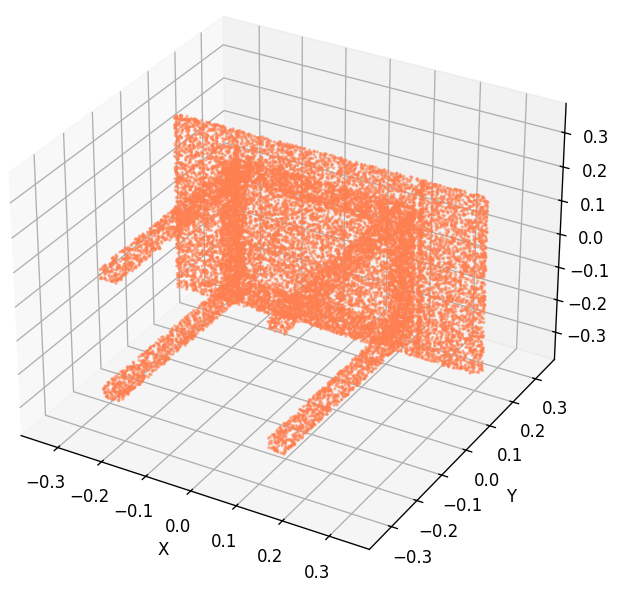
\includegraphics[width=\textwidth]{img/reconstruction_ground_truth.png}
        \caption{Ground Truth}
        \label{fig:recon_gt}
    \end{subfigure}
    \hfill % Adds spacing
    % Second subfigure: Baseline
    \begin{subfigure}[b]{0.32\textwidth}
        \centering
        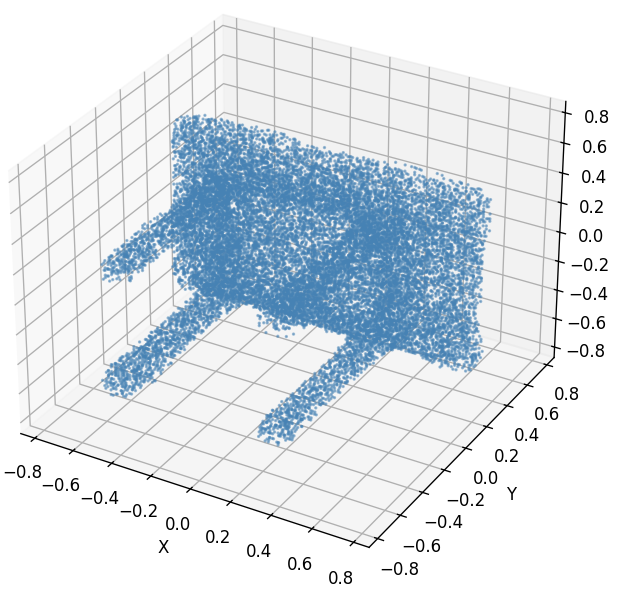
\includegraphics[width=\textwidth]{img/reconstruction_baseline_deepsdf.png}
        \caption{Baseline DeepSDF}
        \label{fig:recon_baseline}
    \end{subfigure}
    \hfill % Adds spacing
    % Third subfigure: Generative
    \begin{subfigure}[b]{0.32\textwidth}
        \centering
        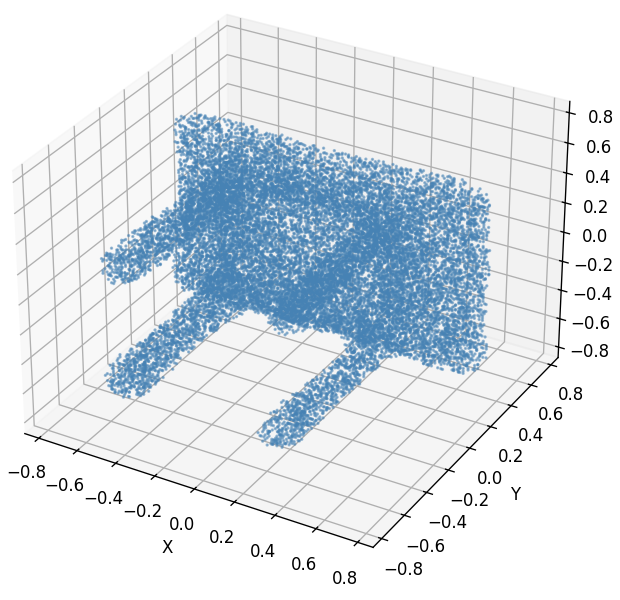
\includegraphics[width=\textwidth]{img/reconstruction_generative_deepsdf.png}
        \caption{Generative DeepSDF}
        \label{fig:recon_ours}
    \end{subfigure}
    
    \caption{Visual comparison of the reconstruction results. (a) Ground-truth geometry. (b) Qualitative outputs from the baseline DeepSDF. (c) Outputs from proposed Generative DeepSDF, demonstrating that high-fidelity details and global topology are preserved despite the discrete VQ bottleneck.}
    \label{fig:visual_comparison}
\end{figure}

As shown in Table~\ref{tab:reconstruction}, the quantitative evaluation indicates that the Generative DeepSDF model exhibits slightly higher values for both Chamfer Distance and Earth Mover's Distance compared to the baseline. This marginal increase in both metrics suggests a minor reduction in numerical reconstruction fidelity, which is an expected trade-off when introducing the discrete Vector Quantization (VQ) bottleneck. However, qualitatively, the reconstructed shapes remain highly consistent with both the baseline and the ground truth. These results demonstrate that the model successfully regularizes the latent space while maintaining a representational capacity that is practically comparable to the continuous baseline.

\subsection{Latent Space Regularization}
The hypothesis of this experiment is that vector quantization will enforce structure on the unconstrained latent manifold. To quantitatively evaluate the structural grouping, the Silhouette Coefficient for the latent codes is compared between both models.

\begin{table}[htbp]
    \centering
    \caption{Evaluation of latent space clustering. Higher values indicate better separation between categorical geometries.}
    \begin{tabular}{lc}
        \hline
        \textbf{Model} & \textbf{Silhouette Coefficient $\uparrow$} \\
        \hline
        Baseline DeepSDF & 0.0522  \\
        \textbf{Generative DeepSDF} & \textbf{0.1298} \\
        \hline
    \end{tabular}
    \label{tab:silhouette}
\end{table}

As shown in Table~\ref{tab:silhouette}, the baseline model exhibits a lower Silhouette Coefficient, indicating poorly defined categorical boundaries. In contrast, Generative DeepSDF achieves a higher value, showing the benefit of forcing the model to select from a learned dictionary of prototypical features.

\begin{figure}[htbp]
    \centering
    % Left side: Ground Truth Samples
    \begin{subfigure}[b]{0.45\textwidth}
        \centering
        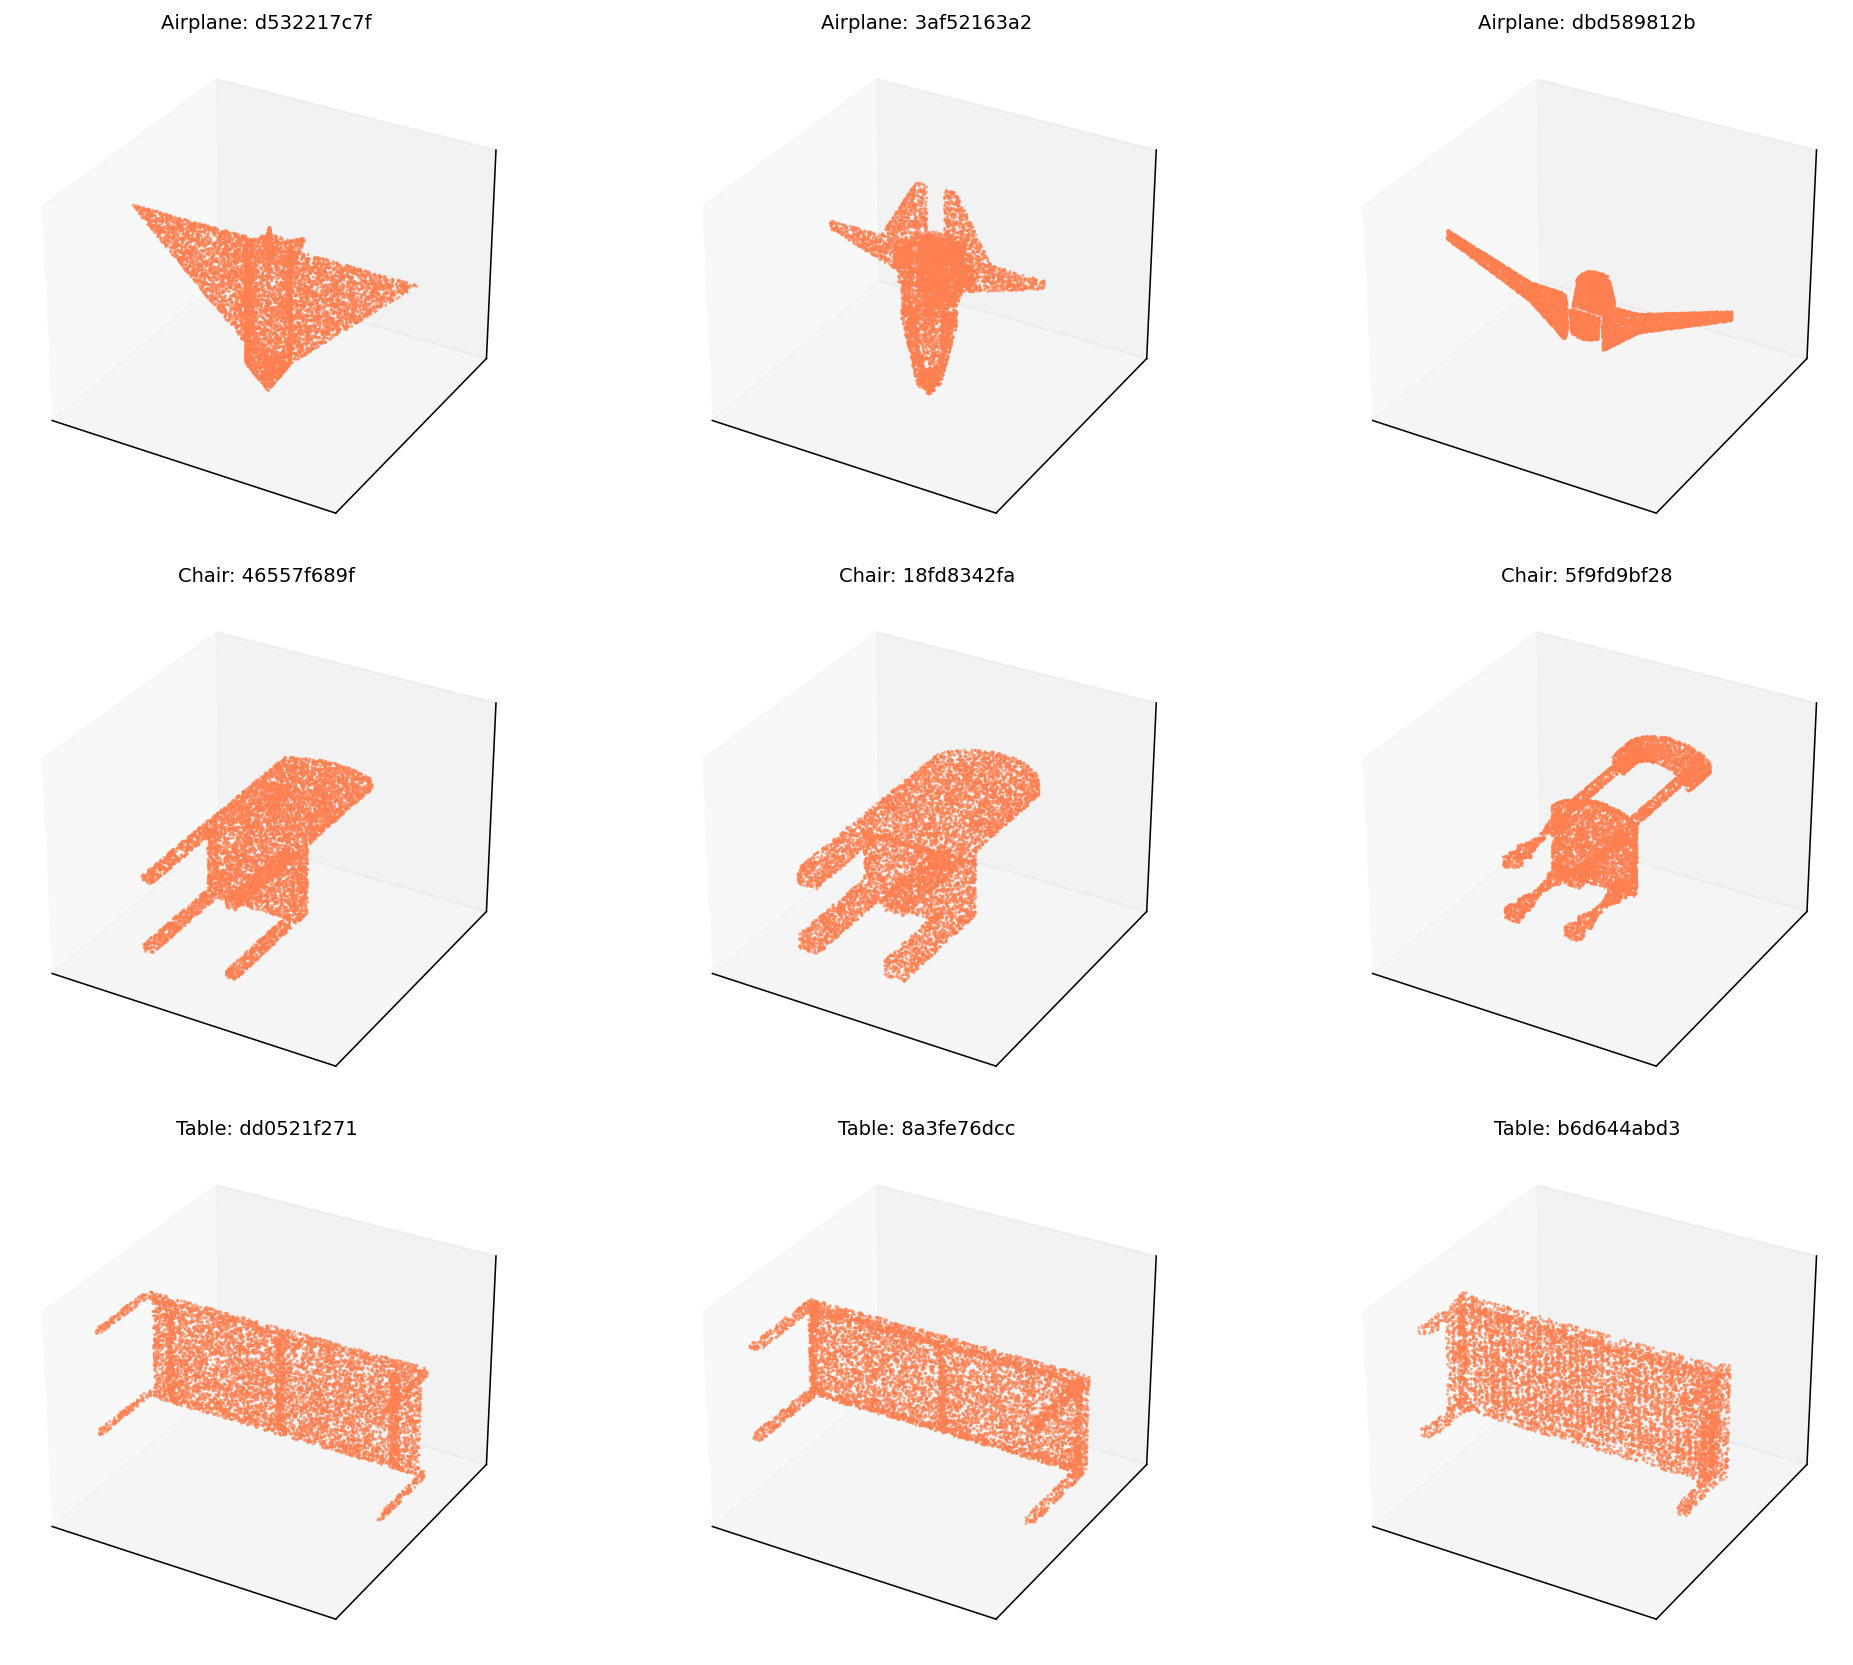
\includegraphics[width=\textwidth]{img/latent_codes_groundtruth.png}
        \caption{Ground truth samples}
        \label{fig:ground_truth}
    \end{subfigure}
    \hfill % Adds spacing between the two images
    % Right side: Latent Code Heatmap
    \begin{subfigure}[b]{0.53\textwidth}
        \centering
        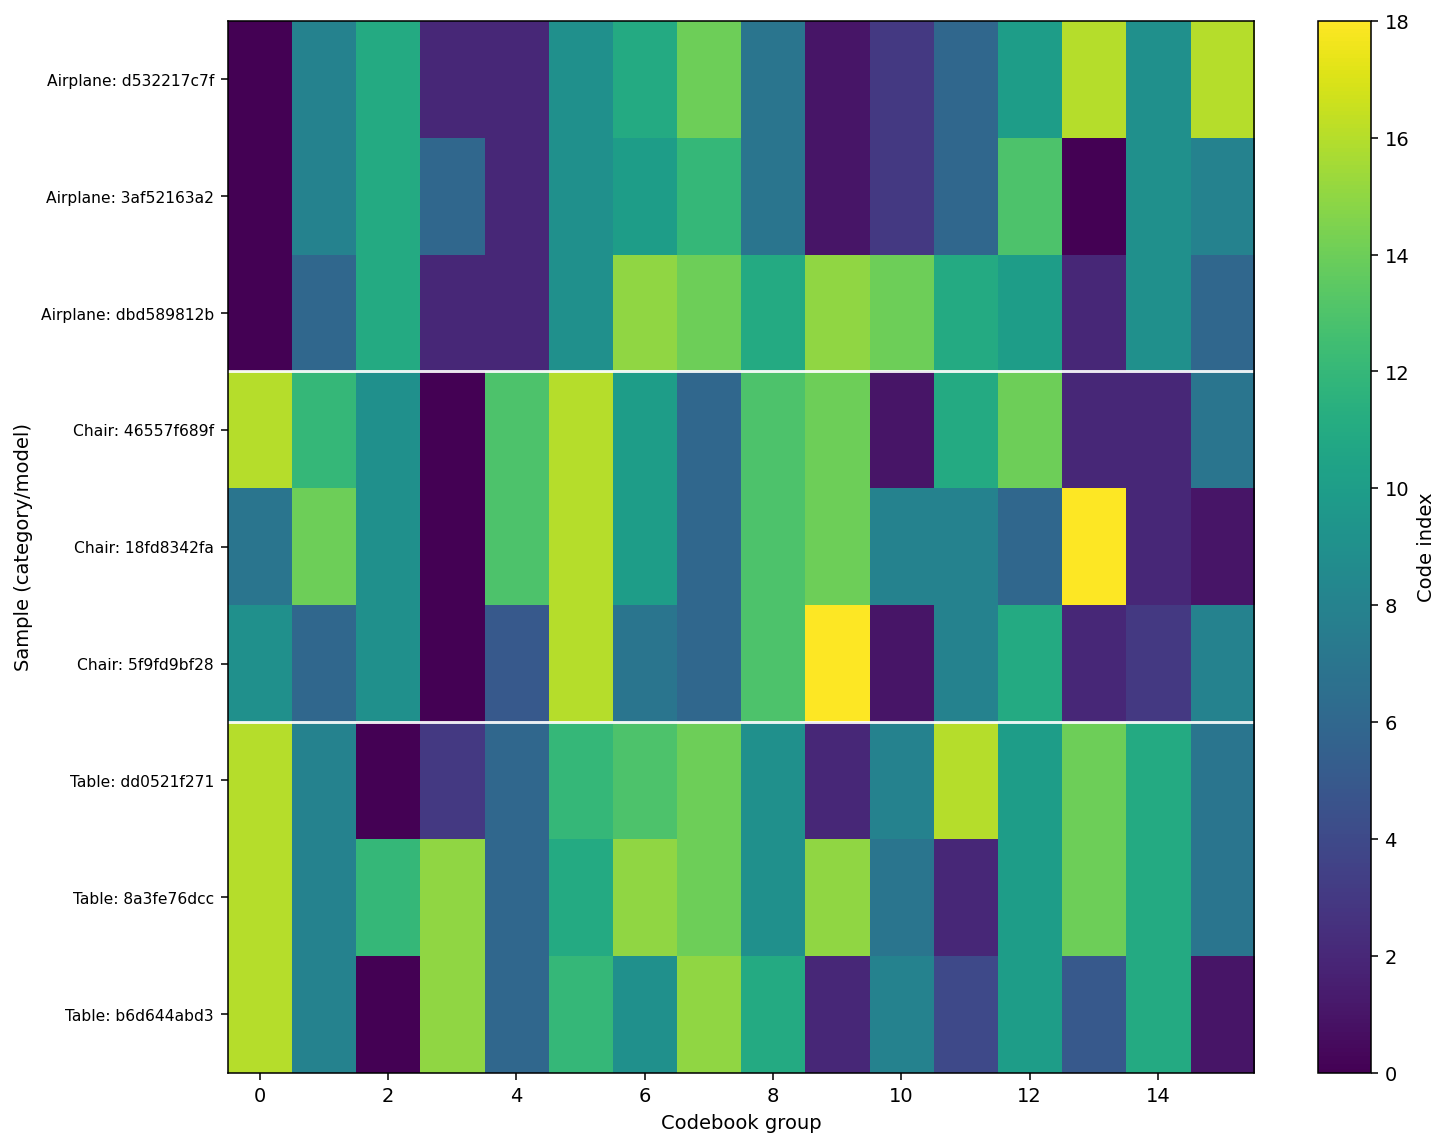
\includegraphics[width=\textwidth]{img/latent_codes.png}
        \caption{Discrete latent code heatmap}
        \label{fig:latent_heatmap}
    \end{subfigure}
    
    \caption{Qualitative analysis of the discrete latent space. (a) shows sample point clouds from three categories, while (b) visualizes the corresponding 16-group VQ latent codes. The consistent patterns within rows of the same category demonstrate successful semantic clustering.}
    \label{fig:combined_latent_analysis}
\end{figure}

Figure~\ref{fig:combined_latent_analysis} provides a qualitative visualization of this structured discrete space. The continuous latent representations are successfully partitioned into fixed-length sequences ($G=16$) of discrete codebook indices. The heatmap in Figure~\ref{fig:combined_latent_analysis}b reveals a high degree of intra-class consistency. Samples belonging to the same category exhibit strikingly similar patterns across the 16 codebook groups. Furthermore, the clear horizontal boundaries between the grouped rows highlight significant inter-class variance. This transition from an unconstrained continuous vector to a structured, categorical sequence confirms the efficacy of the VQ bottleneck and provides the necessary discrete grammar for the autoregressive generative prior.

\subsection{Generative Quality and Novel Synthesis}
A primary advantage of the proposed Generative DeepSDF over traditional auto-decoders is the ability to synthesize novel, physically plausible 3D shapes. This generative capability is evaluated quantitatively using Minimum Matching Distance (MMD).

Baseline novel shapes were generated via random Gaussian sampling while the Generative DeepSDF utilized the 3-layer Autoregressive (AR) Transformer prior to probabilistically sample valid discrete codebook sequences.

\begin{table}[htbp]
    \centering
    \caption{Quantitative evaluation of generative capabilities. Lower Minimum Matching Distance (MMD) values indicate generated shapes more closely resemble the target training distribution.}
    \begin{tabular}{lc}
        \hline
        \textbf{Generation Method} & \textbf{MMD $\downarrow$} \\
        \hline
        Baseline (Random Gaussian Sampling) & 0.3282 \\
        \textbf{Generative DeepSDF (AR Prior)} & \textbf{0.1046} \\
        \hline
    \end{tabular}
    \label{tab:mmd}
\end{table}

As shown in Table~\ref{tab:mmd}, the baseline model struggles with random sampling due to its unconstrained latent space, frequently producing random shapes. Conversely, the AR prior ensures only valid combinations of geometric features are sampled, yielding a superior MMD score. 

\begin{figure}[htbp]
    \centering
    
    % % ==========================================
    % % ROW 1: Dataset Shapes (Ground Truth)
    % % ==========================================
    % \begin{subfigure}[b]{0.32\textwidth}
    %     \centering
    %     \includegraphics[width=\textwidth]{img/dataset_shape_1.png}
    %     \caption{Dataset Sample 1}
    % \end{subfigure}
    % \hfill
    % \begin{subfigure}[b]{0.32\textwidth}
    %     \centering
    %     \includegraphics[width=\textwidth]{img/dataset_shape_2.png}
    %     \caption{Dataset Sample 2}
    % \end{subfigure}
    % \hfill
    % \begin{subfigure}[b]{0.32\textwidth}
    %     \centering
    %     \includegraphics[width=\textwidth]{img/dataset_shape_3.png}
    %     \caption{Dataset Sample 3}
    % \end{subfigure}
    
    % \vspace{0.4cm} % Adds vertical space between rows
    
    % ==========================================
    % ROW 2: Baseline (Gaussian Sampling)
    % ==========================================
    \begin{subfigure}[b]{0.32\textwidth}
        \centering
        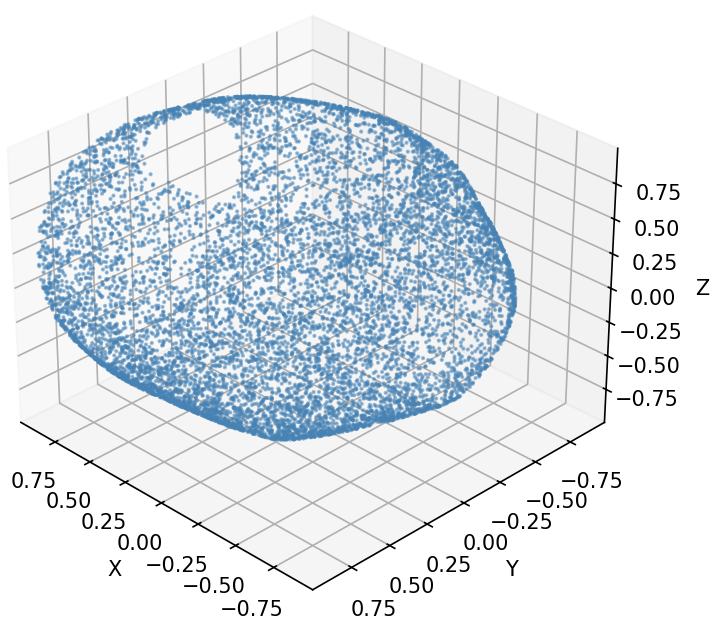
\includegraphics[width=\textwidth]{img/baseline_gen_1.png}
        \caption{Baseline Gen 1}
    \end{subfigure}
    \hfill
    \begin{subfigure}[b]{0.32\textwidth}
        \centering
        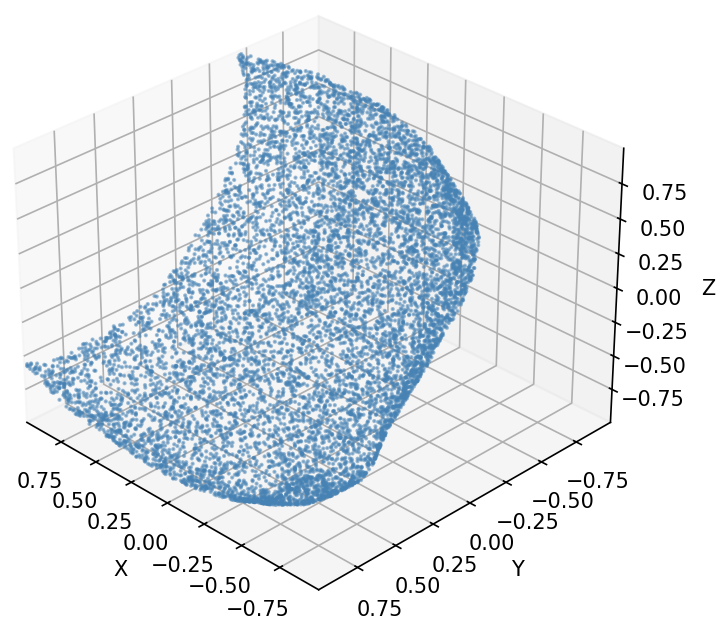
\includegraphics[width=\textwidth]{img/baseline_gen_2.png}
        \caption{Baseline Gen 2}
    \end{subfigure}
    \hfill
    \begin{subfigure}[b]{0.32\textwidth}
        \centering
        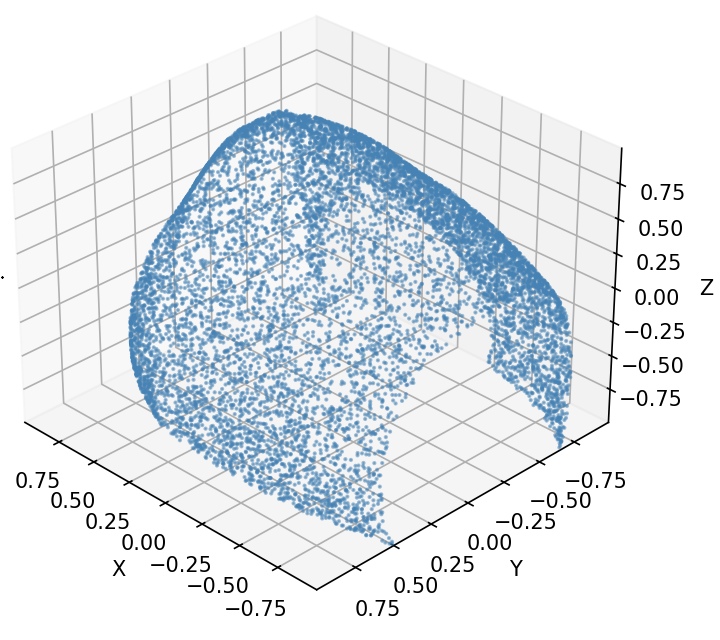
\includegraphics[width=\textwidth]{img/baseline_gen_3.png}
        \caption{Baseline Gen 3}
    \end{subfigure}
    
    \vspace{0.4cm} % Adds vertical space between rows
    
    % ==========================================
    % ROW 3: Generative DeepSDF (AR Prior)
    % ==========================================
    \begin{subfigure}[b]{0.32\textwidth}
        \centering
        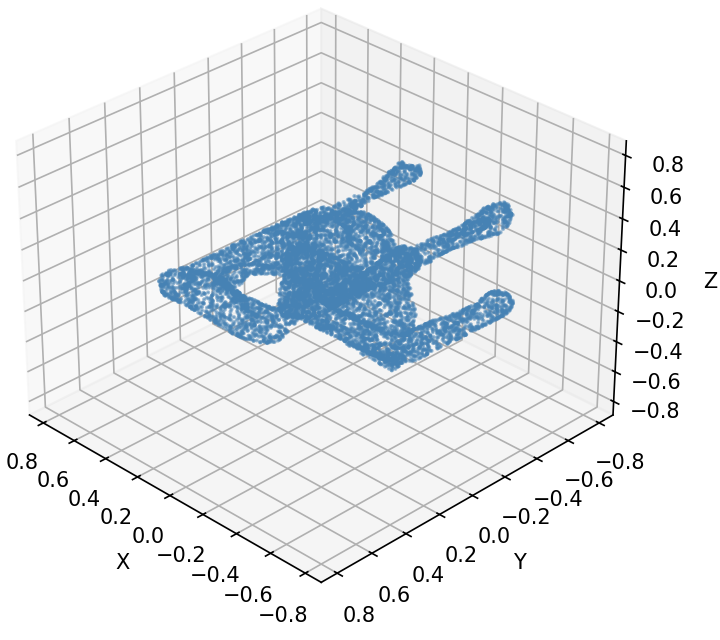
\includegraphics[width=\textwidth]{img/ar_gen_1.png}
        \caption{AR Prior Gen 1}
    \end{subfigure}
    \hfill
    \begin{subfigure}[b]{0.32\textwidth}
        \centering
        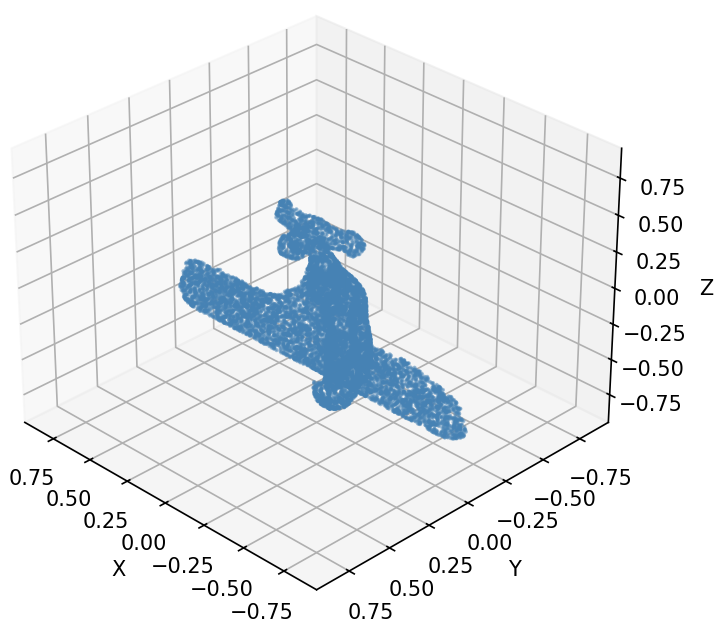
\includegraphics[width=\textwidth]{img/ar_gen_2.png}
        \caption{AR Prior Gen 2}
    \end{subfigure}
    \hfill
    \begin{subfigure}[b]{0.32\textwidth}
        \centering
        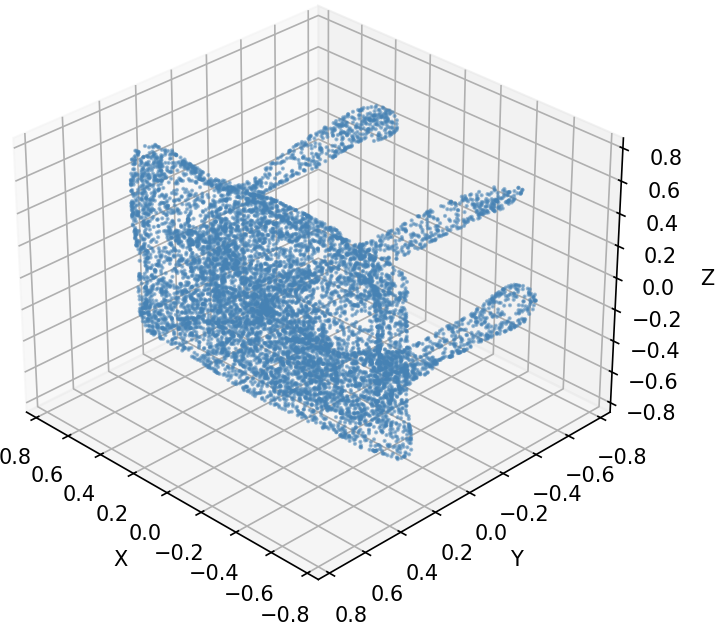
\includegraphics[width=\textwidth]{img/ar_gen_3.png}
        \caption{AR Prior Gen 3}
    \end{subfigure}
    
    \caption{Qualitative comparison of generative capabilities. \textbf{Top Row:} Novel shapes synthesized by the baseline continuous model using random Gaussian sampling, frequently resulting in disconnected artifacts or undefined geometries. \textbf{Bottom Row:} Novel shapes synthesized by the proposed Generative DeepSDF using the discrete AR prior, demonstrating superior structural coherence.}
    \label{fig:generation_grid}
\end{figure}

As illustrated in Figure~\ref{fig:generation_grid}, the baseline model utilizing random Gaussian sampling produces unstructured geometries that fail to capture meaningful object semantics. In contrast, the proposed AR prior synthesizes novel shapes with significantly better structural coherence by sampling valid combinations of learned discrete features.

\section{Conclusion and Future Work}
This report presented Generative DeepSDF, a framework that successfully bridges the gap between deterministic 3D reconstruction and probabilistic shape generation. By integrating a Vector Quantization (VQ) bottleneck into the DeepSDF architecture, the unconstrained latent space was structured into a reusable dictionary of geometric features. This approach maintained strong reconstruction accuracy while enabling a lightweight Autoregressive (AR) prior to generate novel, coherent shapes—significantly outperforming baseline continuous sampling.

While the architectural foundation proved successful, the visual fidelity of the generated shapes remains limited due to hardware constraints that restricted the training dataset to only 150 total objects. Because of this, the model was forced to learn from a limited geometric vocabulary.

Future work will primarily focus on data scaling. Training this framework on large, diverse 3D datasets will naturally enrich the learned codebook, paving the way for high-fidelity shape synthesis. Additionally, future iterations could explore spatially-aware quantization. Instead of compressing an entire shape into a single global 1D sequence, mapping discrete codes to a localized 3D voxel grid could offer finer, part-level control over the generated geometries.

\section{Source Code}
The complete source code is available at the following repository:
\begin{center}
    \url{https://github.com/Ardacandra/ai6131_3d_deep_learning_final_project}
\end{center}

\section{Generative AI Declaration}

The author utilized Github Copilot \cite{githubcopilot} to help with the code implementation and Gemini 3.0 Pro \cite{gemini2026} to provide grammatical refinements and perform technical spell-checking across the report. The core experimental design and the interpretation of the results remain the original work of the author.


% \vspace{5em}
% \newpage
% --- References ---
\bibliographystyle{ieeetr} % or 'plain', 'unsrt', etc.
\bibliography{references}  % Points to references.bib

\end{document}